%%%% PROCESAR con PdfLaTeX !!!!

\documentclass[12pt]{book}

% --------------------------------------------------
% Paquetes
% --------------------------------------------------

\usepackage[top=2cm,bottom=2cm,left=3cm,right=3cm]{geometry}

\usepackage[utf8]{inputenc}
\usepackage[T1]{fontenc}
\usepackage[spanish]{babel}

\usepackage{amssymb}
\usepackage{amsmath}
\usepackage{graphicx}
\usepackage{txfonts}

\usepackage[hidelinks]{hyperref}

% --------------------------------------------------
% Configuración
% --------------------------------------------------

\setcounter{tocdepth}{3}

\hypersetup{
    colorlinks=true,
    linkcolor=black,
    filecolor=magenta,
    urlcolor=cyan,
    pdftitle={Apuntes de Física IA},
    bookmarks=true
}

% --------------------------------------------------
% Documento
% --------------------------------------------------

\begin{document}

% --------------------------------------------------
% Portada
% --------------------------------------------------

\thispagestyle{empty}

\begin{center}

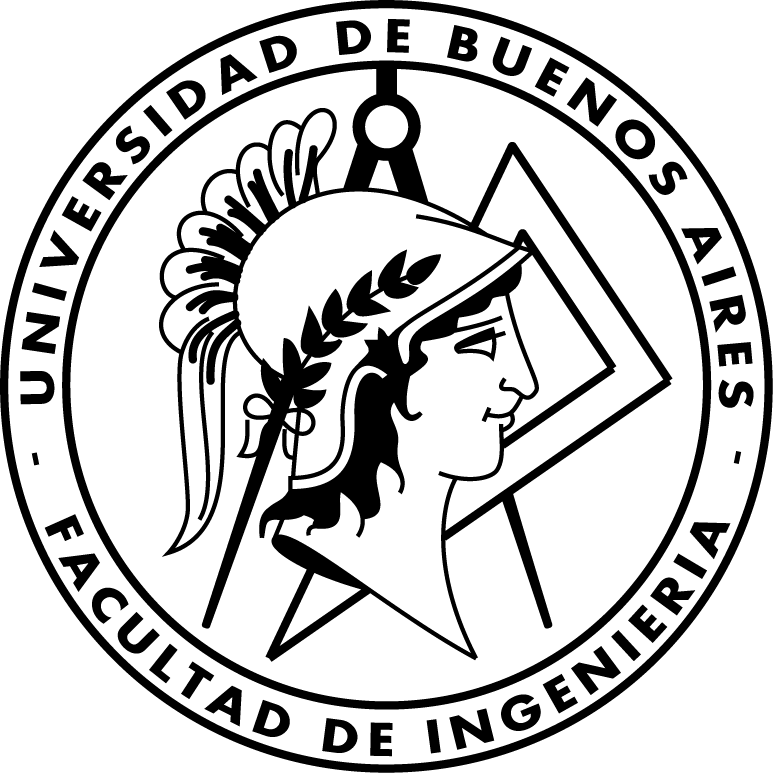
\includegraphics[scale=0.4]{Logo-fiuba_big.png}

\medskip

UNIVERSIDAD DE BUENOS AIRES

Facultad de Ingeniería

Departamento de Física

\vspace{3cm}

\textbf{\large FÍSICA IA -- (62.01)}

\vspace{2cm}

Este es un modesto aporte para los alumnos de la
Facultad de Ingeniería de la UBA, de las carreras de
Licenciatura en Análisis de Sistemas e Ingeniería Informática.

De ninguna manera pretende ser una guía de estudio ni
reemplaza las clases presenciales. El material oficial de
la cátedra está disponible en el sitio web de la materia.

\medskip

\url{http://materias.fi.uba.ar/7510/}

\end{center}

\vspace{2.5cm}

\noindent Autor:\, Isaac Edgar Camacho Ocampo

\noindent Carrera:\, Licenciatura en Análisis de Sistemas

\vspace{1cm}

\noindent Buenos Aires, 2019

\newpage

% --------------------------------------------------
% Índice
% --------------------------------------------------

\tableofcontents

\newpage

% --------------------------------------------------
% Capítulo 1
% --------------------------------------------------

\chapter{¿Qué es la Mecánica?}

En física, se conoce como mecánica al estudio y análisis
del movimiento y reposo de los cuerpos, así como su evolución
temporal bajo la acción de una o varias fuerzas.

\begin{center}
    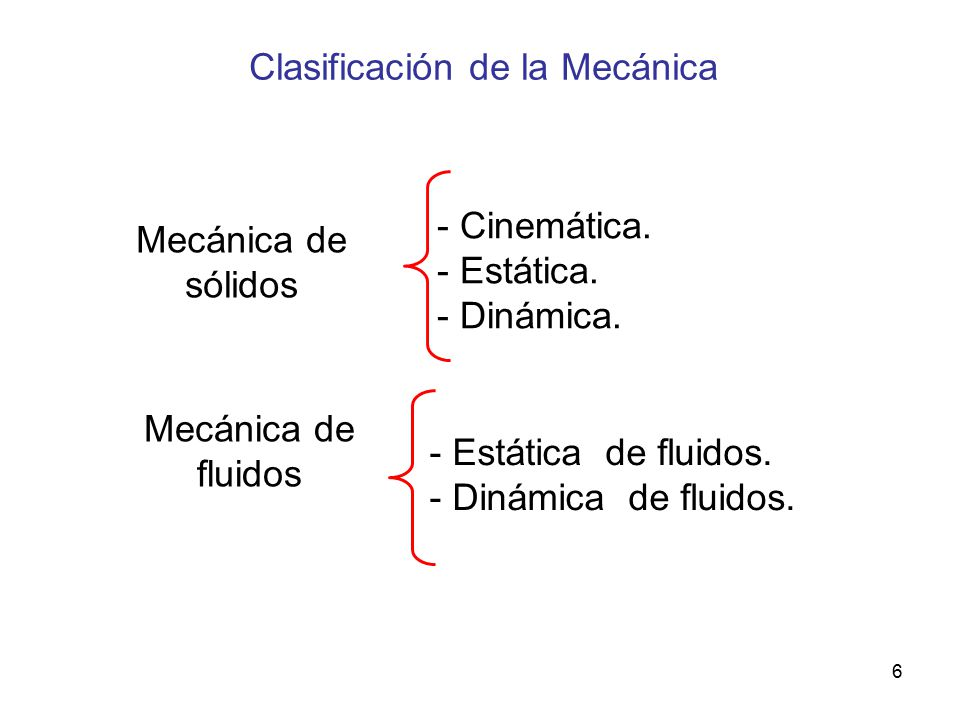
\includegraphics[scale=0.4]{./img/01.jpg}
\end{center}

% --------------------------------------------------

\section{¿Qué es una partícula en física?}

Partícula es un concepto con varios usos. Por lo general,
se emplea para nombrar a una porción de dimensiones muy
reducidas de materia. Un átomo es una partícula.

% --------------------------------------------------

\section{¿Qué es un sistema de referencia en física?}

Un sistema de referencia es un conjunto de coordenadas
espacio-temporales que se requiere para poder determinar
la posición de un punto en el espacio.

Un sistema de referencia puede estar situado en el ojo
de un observador. El ojo puede estar parado o en movimiento.

\begin{center}
    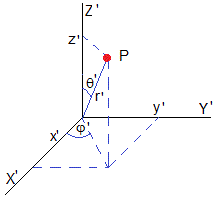
\includegraphics[scale=0.8]{./img/02.png}
\end{center}

% --------------------------------------------------
% Capítulo 2
% --------------------------------------------------

\chapter{Cinemática -- CBC}

La cinemática es la rama de la mecánica que describe el
movimiento de los objetos sólidos sin considerar las causas
que lo originan y se limita, principalmente, al estudio de
la trayectoria en función del tiempo.

\section{Teoría clásica}

\subsection{Definición de variables}

\subsection{Pruebas y refutaciones}

\section{Hipótesis}

% --------------------------------------------------
% Capítulo 3
% --------------------------------------------------

\chapter{Resultados}

\section{Simulación de resultados}

\subsection{Suposiciones}

\subsection{Modelos}

\section{Resultados preliminares}

\section{Resultados postprocesados}

\subsection{Valores atípicos}

\subsection{Correlaciones}

% --------------------------------------------------
% Capítulo 4
% --------------------------------------------------

\chapter{Conclusiones}

\end{document}
```
